% Metódy inžinierskej práce
%Vojtech Babinský, 120750, 2022

\documentclass[10pt,oneoside,slovak,a4paper]{article}

\usepackage[slovak]{babel}
%\usepackage[T1]{fontenc}
\usepackage[IL2]{fontenc} % lepšia sadzba písmena Ľ než v T1
\usepackage[utf8]{inputenc}
\usepackage{graphicx}
\usepackage{url} % príkaz \url na formátovanie URL
\usepackage{hyperref} % odkazy v texte budú aktívne (pri niektorých triedach dokumentov spôsobuje posun textu)

\usepackage{caption}

\usepackage{cite}
%\usepackage{times}

\newcommand{\source}[1]{\caption*{Source: {#1}} }

%použil som príkaz z nasledujúceho linku na pridanie zdroja k obrázku
%https://tex.stackexchange.com/questions/95029/add-source-to-figure-caption

%TO DO:
% SKRATIT ABSTRAKT








\pagestyle{plain}

\title{Hry o prežitie\thanks{Semestrálny projekt v predmete Metódy inžinierskej práce, ak. rok 2022/2023, vedenie: Vladimír Mlynarovič}} % meno a priezvisko vyučujúceho na cvičeniach

\author{Vojtech Babinský\\[2pt]
	{\small Slovenská technická univerzita v Bratislave}\\
	{\small Fakulta informatiky a informačných technológií}\\
	{\small \texttt{xbabinskyv@stuba.sk}}
	}

\date{\small 6. november 2022} % upravte



\begin{document}

\maketitle

\begin{abstract}

Vďaka pokroku, sa už väčšina populácie v rozvinutých krajinách nemusí zaoberať poľnohospodárstvom, lovom, zberom a podobnou ťažkou fyzickou prácou. Tieto aktivity, dnes vykonáva, vzhľadom na ostatok obyvateľstva, len hŕstka ľudí. 

Niektorí ľudia, však vo svojom voľnom čase siahajú po hrách simulujúcich tieto činnosti, často v extrémnych podmienkach, kde každá chyba môže mať nemilý vplyv na ďalšie hranie. Ide teda o špecifický prípad, kde na rozdiel od väčšiny iných hier, hráč nie je nezraniteľným hrdinom, ale súčasťou prostredia, v ktorom zápasí s hladom, zvieratami/príšerami, počasím, inými hráčmi atď. 

Cieľom článku je zoznámiť čitateľa s tzv. hrami o prežite (ang. Survival games).Pokúsi sa opísať kritéria, ktoré musia hry spĺňať, aby mohli byť zaradené do tohto žánru, poskytne príklady  úspešných herných predstaviteľov tejto kategórie a predstaví aj jej rôzne subžánre. 
\end{abstract}


\newpage

\section{Úvod}
Počítačové hry sú relatívne nová forma zábavy, ktorej vývoj kopíruje rozvoj a dostupnosť počítačov. Tak ako v literatúre, jestvuje mnoho rozličných žánrov a hranice medzi nimi hier sú pružné.To znamená, že niektoré hry teda môžu byť zaradené do viacerých naraz. V tomto článku sa budem zaoberať „hrami o prežitie“ (alebo aj survival hrami ). 

Ako už napovedá sám názov tohto druhu hier, dôležitou je snaha prežiť. Základnou črtou survival hier je hospodárenie so surovinami, často zahrňujúce výrobu (crafting) a recykláciu, pomocou, ktorých dokážete svoju postavu dlhšie udržať pri živote. \cite{Pavlovic}

Ďalším znakom je možnosť zranenia sa (prejavuje sa ako dočasné znevýhodnenie hráča), prípadne smrti v hre. 

Tá môže nastať po konfrontácii s inými ľuďmi, zvieratami a príšerami, čo tiež patrí medzi základne elementy hier o prežitie.\cite{Reid}

\section{História hier o prežitie }

\begin{figure}[h]
	\begin{flushleft}
		
		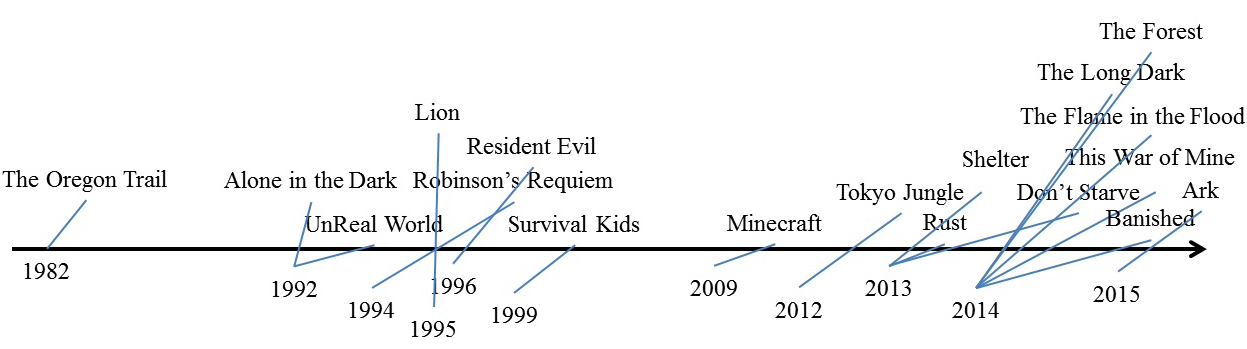
\includegraphics[width=12.5cm,keepaspectratio]{REID_graf.png}
		\caption{\textit{Časová os vzniku žánru videohier s tematikou prežitia}}
		\label{ fig:Časová os vzniku žánru videohier s tematikou prežitia}
  		\caption*{Zdroj: Reid (2018). \cite{Reid}}
		
	\end{flushleft}
\end{figure}

Prvou komerčne úspešnou survival hrou bola The Oregon trail, vydaná v 80tych rokoch minulého storočia. Jej úplne prvá verzia, však uzrela svetlo sveta v roku 1971. 

Dan Rawitsch, vtedy 21 ročný vysokoškolák a učiteľ , dostal za úlohu učiť žiakov 8. triedy históriu americkej expanzie na západ. Chcel urobiť niečo nové a interaktívne, a preto pre svojich žiakov vytvoril stolnú hru. \cite{Toppo}

Keď jeho spolubývajúci, učiteľ matematiky,  Bill Heinemann videl mapu tejto hry povedal Rawitschovi, že by to mohol byť perfektný program pre počítač. Ukázal mapu ďalšiemu spolubývajúcemu Paulovi Dillenbergerovi, ktorý tiež učil matematiku. Tomu sa nápad zapáčil a pustili sa do diela. 

Základ hry je cestovanie so skupinkou osadníkov z mestečka Independence (štát Missouri) do štátu Oregon na východe  USA.

V úvode si hráč nakúpi zásoby jedla, náboje a zvieratá na cestu.  Počas výpravy musí prekonať rôzne náhodné udalosti ako rozbitie kolesa na voze, uhryznutie hadom a choroby.

Hra nemala žiadnu grafiku a bola čisto textová, jej kód mal 800 riadkov a bola naprogramovaná v jazyku BASIC. Ihneď sa stala hitom medzi študentmi školy, ktorí stáli v radoch aby si mohli zahrať. 

Hoci po vydaní The Oregon Trail nasledovala dekáda útlmu popularity survival hier \ref{ fig:Časová os vzniku žánru videohier s tematikou prežitia},tento žáner prešiel obrovským vývojom a dnes patrí medzi najobľúbenejšie. \cite{IGN}


\section{Subžánre} 
Survival hry majú dva hlavné subžánre – Wilderness survival (prežitie v divočine) a Survival  horror.  Samozrejme, jestvuje mnoho hier, pri ktorých nie je jednoduché zaradiť ich do jednej z dvoch predstavených skupín, voláme ich preto vznikajúce typy (alebo aj hybridy).\cite{Reid}

\subsection{Wilderness survival}

Hry tohto subžánru, sa sústredia na schopnosti prežitia v prírode. Hráč zvyčajne začína ako lovec a zberač. Postupným hraním si vyrobí nástroje a zbrane a nájde úkryt, z ktorého vychádza na výpravy. Do tejto skupiny hier patrí napríklad už spomenutá The Oregon Trail, The Long Dark a Unreal World.\cite{Wilds}

\subsubsection{UnReal world}
Prvýkrát vyšla v roku 1992. Je to práca dvoch ľudí, hlavného vývojára Samiho Maaranena a Errku Lehmusa. Pôvodne to bola fantasy RPG hra, ktorá sa postupne vyvinula na Wilderness survival situovaný v dnešnom Fínsku v dobe železnej. 

Hráč sa pohybuje v masívnom náhodne generovanom svete s jediným cieľom - prežiť čo najdlhšie. Musí si pritom dávať pozor na zimu, hlad,únavu... Level realizmu je naozaj vysoký.

UnReal world je držiteľom dvoch rekordov: je to najdlhšie podporovaná hra na svete a prvá survival hra s otvoreným svetom. \cite{UnRealWorld}

\subsubsection{The Long Dark}

Táto survival hra z roku 2014, sa odohráva v zimnej a drsnej kanadskej divočine. The Long Dark ponúka survival mód a príbehový mód s názvom Wintermute.

Survival mód sa  sústrďuje iba na samo prežitie, ide o sandbox  mód (hráč má voľnú ruku v tom ako chce hrať).  Samozrejme, hra ponúka  možnosť získania rôznych úspechov (achievementov), ktoré môžu motivovať ľudí k ďalšiemu hraniu. \cite{Virtanen}

V príbehovom móde hráč striedavo hrá za pilota Willa Mackenzieho  alebo doktorku  Astrid Greenwoodovú. Počas spoločného letu svet postihla nevysvetlená katastrofa, ktorá zapríčinila pád ich lietadla. Cieľom hráča je priviesť oboch hrdinov ku sebe a odhaliť dôvod katastrofy. \cite{Virtanen}

Momentálne sú dostupné štyri kapitoly príbehu, pričom záverečná piata je vo vývoji.


\subsection{Survival Horror}
Pojem Survival horror sa prvýkrát objavil v hre Resident evil, a odvtedy sa používa na označenie hier tohto typu. \cite{Kirkland} Tieto hry kombinujú silný emočný zážitok hororových filmov s mechanikami hier o prežitie.Strach a pocit napätia u hráča vyvoláva často  tmavé prostredie, hudba a rozličné príšery.

\subsubsection{Resident Evil}
Japonská herná séria Resident Evil (v Japonsku známa pod názvom Biohazard \cite{Capcom}), patrí medzi najpopulárnejšie tohto subžánru. Od roku 1996 vrátane, vyšlo desať hlavných hier, hoci spolu s rôznymi vedľajšími by to mohlo byť okolo tridsať.  \cite{ResEv}

Dej hry sa začína vyslaním druhého špeciálneho oddielu, ktorý má zistiť príčinu objavenia sa v meste Racoon brutálnych kanibalov. Na svojej výprave rýchlo zistia, že helikoptéra prvého tímu havarovala a objavia obrovskú vilu plnú hrôzostrašných stvorení...\cite{WindowsCentral}

Okrem hier vyšlo aj sedem filmov Hollywoodskej produkcie. Filmy zo série Resident Evil sú najviac zarábajúcimi stvárneniami počítačových hier. \cite{Ehli}


\subsubsection{Alone in the dark}
Prvý diel tejto série sa dostal na trh v roku 1992. Ide o point and click adventúru, čiže hráč ovláda postavu prevažne klikaním na objekty. Najefektívnejší spôsob konfrontácie hráča s príšerami, je jednoducho vyhýbať sa im.\cite{Reid}

Príbeh sa začína, po tom ako súkromný bol vyšetrovateľ Edward Carnby najatý na nájdenie vzácneho piana vo ville umelca Jeremyho Artwooda, ktorý spáchal samovraždu za nevyjasnených okolností. Po vstúpení do tejto vily, ktorá mala reputáciu prekliatej, sa dvere uzamknú a Edward ostane uväznený. Vzápätí ho prepadnú monštrá a zabránia mu vystúpiť na povalu, kde by sa malo nachádzať vzácne piano.\cite{Swan}

Momentálne je vo vývoji, nová  rovnomenná hra od svetoznámeho vydavateľa THQ Nordic, ktorá je inšpirovaná originálom z roku 1992.\cite{Alone}

\subsubsection{Project Zomboid}

Táto  hra začala ako projekt štyroch nezávislých vývojárov, ktorých cieľom bolo vyvinúť čo najlepšiu zombie survival hru. Hra má retro grafický štýl, kameru zobrazujúcu prostredie z izometrickej perspektívy a mnoho malých detailov.\cite{Mosel}

Project Zomboid bol vydaný v roku 2013 a recenzie hráčov na stránke Steam sú veľmi kladné.\cite{Zomboid}

Dej sa odohráva v Muldraug, okres Knox  v štáte Kentucky. Celá oblasť bola uzavretá v karanténe z dôvodu zamorenia zombíkmi.  Hlavný hrdina Bob ostal uväznený v zóne spolu so svojou ženou Kate, ktorá mala poranenú nohu a nemohla chodiť.
Čím dlhšie hráč prežíva, tým viac znakov zániku civilizácie vidí. Od popraskaného asfaltu po konečný výpadok elektriny. 

Hra nemá vyložený cieľ, ktorý keď hráč splní tak vyhrá. Neodvratným koncom je smrť, ktorá môže nastať z rôznych príčin, od boja s nakazenými po konfrontáciu s banditmi.\cite{Mosel}







\subsection{Hry hybridného žánru}

Ako už bolo spomenuté, niekedy nie je možné  jednoznačne zaradiť hru do žánru hier o prežitie . Hry, ktoré spájajú klasické atribúty survival hier s rôznymi inými žánrami nazývame „hybridnými“. 

\subsubsection{This war of mine}

Hra poľského vývojára 11bit Studios bola inšpirovaná skutočnými udalosťami, hlavne Varšavským povstaním, obliehaním Grozného a vojnou v Sýrii. Dostupná pre hráčov je od roku 2014.\cite{PL}

Hra sa odohráva vo  vojnou zmietanom meste. Hráč sa spolu so skupinou ďalších ľudí snaží prežiť obliehanie. Každý z členov skupiny má ukazovateľ hladu, únavy a šťastia. V hre sa strieda deň a noc, pričom obe fázy majú vplyv na hranie. Kým cez deň môže hráč zadávať úlohy ostatným  postavám, v noci je čas na zber materiálu, jedla a vzácností.
Hráč sa tiež nevyhne ťažkým rozhodnutiam. Problémy väčšinou nemajú jednoznačne dobré riešenia, čo ešte viac zvýrazňuje ťažký život civilistov.\cite{Pergerson}

This war of mine, na rozdiel od väčšiny hier s vojnovou tématikou, ukazuje často zabudnutý ťažký život civilistov žijúcich v oblasti postihnutej konfliktom. Práve vďaka silnému protivojnovému odkazu bola hra zaradená  medzi odporúčané materiály v poľskom školstve. \cite{PL}

\subsubsection{Frostpunk}

V roku 2018 sa spoločnosť 11bit Studios zaslúžila o ďalšiu zaujímavú survival hru. Frostpunk spája citybuilder (hry, kde hráč stavia mesto alebo kolóniu) a survival hry. Tematika hry je steampunková (Steampunk je subžánrom sci-fi, ktorý je charakteristický zmiešaním modernej technológie s parným pohonom).\cite{Salo}

Dej sa odohráva na území Anglicka v roku 1887, po tom ako výbuch sopky zapríčinil rapídny pokles teploty na Zemi.
Hráč vystupuje v roli starostu mestu a jeho úlohou je mesto stabilizovať a rozvinúť, napriek neustále klesajúcej teplote. Popritom  musí rozhodovať o zákonoch, ktoré sú často problematické ako napríklad detská práca, pridávanie pilín do jedla a mnohé iné.\cite{Salo}\cite{FW}


\subsubsection{Minecraft}
Táto hra bola vyvíjaná pôvodne jedným človekom Markusom Perssonom a bola vydaná v roku 2009. Hra obsahuje možnosť hrania osamote (single-player) alebo s inými hráčmi (multi-player).
Režim single-player má dva režimy: survival prežitie a creative .
%Dopísať Minecraft !!!!!!

\section{Vyjadrenie sa k témam prednášok} 


\section{Záver} \label{zaver} % prípadne iný variant názvu



%\acknowledgement{Ak niekomu chcete poďakovať\ldots}

\newpage
% týmto sa generuje zoznam literatúry z obsahu súboru literatura.bib podľa toho, na čo sa v článku odkazujete
\bibliography{literatura}
\bibliographystyle{plain} % prípadne alpha, abbrv alebo hociktorý iný

\end{document}
